%%
%% Paper 2 — Mechanistic Understanding of Tabular Transformer Limitations
%% Target venue: Neural Networks (Elsevier)
%%

\documentclass[a4paper,fleqn]{cas-sc}

\usepackage[authoryear,longnamesfirst]{natbib}
\usepackage{booktabs}
\usepackage{multirow}
\usepackage{xcolor}
\usepackage{colortbl}
\usepackage{amsmath}
\usepackage{graphicx}
\usepackage{enumitem}
\usepackage{capt-of}  % \captionof for non-floating tables and figures

%% Consistent model colours (match thesis figures)
\definecolor{clrLGBM}{HTML}{1f77b4}
\definecolor{clrCB}{HTML}{d62728}
\definecolor{clrRF}{HTML}{2ca02c}
\definecolor{clrFT}{HTML}{ff7f0e}
\definecolor{clrLR}{HTML}{9467bd}

\begin{document}
\let\WriteBookmarks\relax
\def\floatpagepagefraction{1}
\def\textpagefraction{.001}

%% ─── Front matter ──────────────────────────────────────────────────────────

\shorttitle{Tabular Transformer Limitations in Financial Fraud Detection}

\shortauthors{Caixeiro et al.}

\title[mode=title]{Mechanistic Understanding of Tabular Transformer Limitations
  in Financial Fraud Detection:
  Cross-Domain Robustness, Foggy Vision Attention, and SHAP Feature Stability}

\author[1]{Olavo Caixeiro}[
  orcid=0009-0004-1532-4830,
]
\cormark[1]
\ead{200100274@esg.ipsantarem.pt}
\credit{Conceptualization, Methodology, Software, Formal analysis, Writing -- original draft}

\author[1]{Maryam Abbasi}[
  orcid=0000-0002-9011-0734,
]
\ead{maryam.abbasi@esg.ipsantarem.pt}
\credit{Conceptualization, Supervision, Writing -- review \& editing}

\author[1]{Pedro Martins}[
  orcid=0000-0001-9600-082X,
]
\ead{pedro.martins@esg.ipsantarem.pt}
\credit{Supervision, Writing -- review \& editing}

\affiliation[1]{
  organization={Departamento de Inform\'atica e M\'etodos Quantitativos,
    Escola Superior de Gest\~ao e Tecnologia,
    Instituto Polit\'ecnico de Santar\'em},
  city={Santar\'em},
  country={Portugal}
}

\cortext[1]{Corresponding author}

%% ─── Abstract ──────────────────────────────────────────────────────────────

\begin{abstract}
Gradient-boosted decision trees routinely match or outperform tabular transformer
models on financial fraud detection benchmarks, yet the mechanisms behind this
empirical regularity are poorly understood.
This paper provides a mechanistic account through four complementary analyses
conducted on the Bank Account Fraud (BAF) suite of six distributional variants.
First, we compare the imbalance-strategy sensitivity of FT-Transformer and CatBoost
across seven resampling and cost-sensitive interventions: SMOTE reduces FT-Transformer
PR-AUC by $41\%$ on BAF but only $14\%$ for CatBoost, revealing an architectural
fragility rooted in the attention mechanism's exposure to synthetic feature
distributions.
Second, we conduct a zero-shot cross-domain transfer experiment (BAF Base
to Variants~I--V) and find that Random Forest improves its PR-AUC on four of five
variants relative to its in-domain score, while all other models --- including
FT-Transformer --- degrade; we attribute this to random feature subsampling acting
as a structural regularizer against domain-specific feature co-occurrence patterns.
Third, Jaccard analysis of SHAP top-10 feature rankings shows that LGBM's feature
attribution is perfectly stable across all six BAF datasets (Jaccard\,$=\,1.00$),
isolating the source of cross-domain performance degradation to the decision
surface rather than the features themselves.
Fourth, attention diagnostics on $200\,000$ BAF test samples reveal a Foggy Vision
pattern (normalised entropy $H_{\text{norm}}\,=\,0.976$), ruling out all
pathological attention behaviours and confirming that the $0.18$~PR-AUC ceiling
reflects the information content of the BAF feature space rather than any
architectural failure.
Convergent evidence from the two independent methods --- attention weights and SHAP
values --- identifies the same three features as the primary fraud signals, providing
cross-method validity for the explanation infrastructure.
Together, the four findings explain why gradient-boosted trees generalise better
than tabular transformers under distribution shift and guide practitioners toward
robust, interpretable, and deployment-ready fraud detection pipelines.
\end{abstract}

\begin{highlights}
\item FT-Transformer PR-AUC drops $41\%$ under SMOTE on BAF vs.\ only $14\%$ for CatBoost
\item Random Forest improves on $4$ of $5$ BAF cross-domain variants despite lower in-domain score
\item LGBM SHAP top-10 feature ranking is identical across all six BAF datasets (Jaccard\,$=\,1.00$)
\item Attention normalised entropy of $0.976$ (Foggy Vision) rules out all pathological attention patterns
\item Top attention tokens and top SHAP features converge, providing cross-method validity for explanations
\end{highlights}

\begin{keywords}
fraud detection\sep
gradient-boosted trees\sep
FT-Transformer\sep
cross-domain generalisation\sep
attention diagnostics\sep
SHAP\sep
class imbalance\sep
distribution shift
\end{keywords}

\maketitle

%% ─── 1. Introduction ────────────────────────────────────────────────────────

\section{Introduction}
\label{sec:intro}

Financial fraud inflicts substantial economic harm globally, and the automated
detection of fraudulent transactions has become a canonical benchmark for
machine learning under extreme class imbalance~\citep{rymantubb2018survey,hilal2022financial}.
The emergence of transformer-based architectures for tabular data --- in particular
the Feature Tokenizer Transformer (FT-Transformer) of~\citet{gorishniy2021revisiting}
--- has raised the question of whether attention-based models offer systematic
advantages over the gradient-boosted decision trees (GBDTs) that have
long dominated tabular prediction tasks~\citep{shwartzziv2022tabular,grinsztajn2022tree}.
A companion study~\citep{caixeiro2025threshold} established that, on two structurally
distinct fraud benchmarks, CatBoost and LGBM match the FT-Transformer in-domain,
and that the choice of decision threshold is a more consequential design variable
than the choice of model.
That finding raises three mechanistic questions that the companion paper, by design,
does not address:
(i) \emph{Why} does FT-Transformer's parity with GBDTs break down under certain
resampling interventions?
(ii) Which model family is most robust when the model trained on one distribution
is deployed on a shifted one --- a routine scenario in production fraud systems?
(iii) Do feature attribution methods agree across architecturally different models
and across distributional shifts, and what does that agreement (or disagreement)
imply about the underlying signal structure?

Existing literature on tabular deep learning vs.\ GBDTs focuses overwhelmingly
on in-distribution accuracy comparisons~\citep{borisov2022deep,gorishniy2022embeddings}
and rarely examines the \emph{mechanism} behind the accuracy gap or its
persistence under distribution shift.
On the interpretability side, SHAP~\citep{lundberg2017unified} has been applied
to individual fraud detection models, but systematic cross-model and cross-domain
Jaccard analysis --- which tests whether independent architectures converge on the
same feature signals --- has not been reported in the fraud literature.
Attention diagnostics, while studied in NLP~\citep{vaswani2017attention}, have
not been applied to fraud tabular data to distinguish dataset-ceiling effects from
architectural pathologies.

This paper addresses all three gaps through four focused analyses on the BAF suite:
\begin{enumerate}[label=C\arabic*.]
  \item \textbf{Imbalance sensitivity}: A direct comparison of FT-Transformer and
    CatBoost across seven class imbalance strategies on two datasets, identifying
    the intervention that exposes the transformer's architectural fragility.
  \item \textbf{Cross-domain robustness}: Zero-shot transfer from BAF Base to
    five distributional variants, revealing an unexpected RF superiority pattern
    and its structural explanation.
  \item \textbf{SHAP cross-model and cross-variant stability}: Jaccard analysis
    of top-$10$ feature attributions across four model families and across
    all six BAF datasets, separating feature stability from decision-surface stability.
  \item \textbf{Attention diagnostics}: A four-pattern diagnostic framework
    applied to $200\,000$ BAF samples, culminating in the Foggy Vision
    interpretation and convergent validity with SHAP.
\end{enumerate}

The rest of the paper is structured as follows.
Section~\ref{sec:related} reviews related work on tabular deep learning,
distribution shift in fraud, and attribution interpretability.
Section~\ref{sec:setup} describes the experimental setup.
Sections~\ref{sec:results}--\ref{sec:discussion} present and interpret the results.
Section~\ref{sec:conclusion} concludes.

%% ─── 2. Related Work ────────────────────────────────────────────────────────

\section{Related Work}
\label{sec:related}

\subsection{Tabular Deep Learning vs.\ Gradient-Boosted Trees}

The ascent of GBDTs as the dominant method on tabular benchmarks --- driven by
LightGBM~\citep{ke2017lightgbm} and CatBoost~\citep{prokhorenkova2018catboost}
--- was challenged by a wave of deep learning models designed for tabular data,
including TabTransformer~\citep{huang2020tabtransformer}, SAINT~\citep{somepalli2021saint},
and FT-Transformer~\citep{gorishniy2021revisiting}.
Empirical evaluations, however, have repeatedly found that these gains are
limited or benchmark-specific.
\citet{shwartzziv2022tabular} benchmark several recent tabular deep learning models
against XGBoost on multiple datasets and find that the tabular DL advantage
is inconsistent, appearing mainly on large numerical-feature datasets.
\citet{grinsztajn2022tree} provide a detailed analysis of the conditions under
which tree-based models outperform deep learning on tabular data, highlighting
irregular decision boundaries and the preponderance of uninformative features as
key factors --- both of which are endemic to fraud detection.
The FT-Transformer's own evaluation~\citep{gorishniy2021revisiting} shows
marginal improvements over CatBoost on some benchmarks, but the gains disappear
or reverse on datasets with categorical-heavy feature spaces, which BAF exemplifies.
\citet{borisov2022deep} survey the field and note that the advantage of deep
learning over tree ensembles on tabular data is not yet established,
particularly under distribution shift or with limited labelled data.

Despite this empirical evidence, the \emph{mechanisms} that drive GBDT advantages ---
especially under class imbalance interventions and distribution shift ---
have received little attention.
This paper fills that gap by examining why the FT-Transformer is systematically
more sensitive to SMOTE than CatBoost and why Random Forest, a simpler ensemble,
outperforms attention-based and boosted models in cross-domain transfer.

\subsection{Distribution Shift and Cross-Domain Robustness in Fraud Detection}

Production fraud detection systems face continuous distribution shift:
fraud patterns evolve as fraudsters adapt to defences, and models trained
at one institution are frequently deployed in new environments~\citep{dalpozzolo2017realistic,rymantubb2018survey}.
\citet{jesus2022turning} introduce the BAF suite specifically to address the
lack of controlled shift benchmarks in fraud detection, offering five variants
with calibrated degrees of covariate shift, label shift, and bias injection.
Their evaluation focuses on in-domain performance and fairness metrics; cross-model
cross-domain robustness analysis is left as an open problem.
\citet{hoppner2021idcs} study temporal distribution shift in credit card fraud
and find that models retrained on recent data degrade less than static models,
but do not compare model families' inherent robustness.
The question of \emph{which} model architecture is structurally more robust
to distribution shift --- GBDTs, random forests, or tabular transformers ---
has not been directly addressed on fraud data.

\subsection{Interpretability: SHAP and Attention as Complementary Tools}

SHAP~\citep{lundberg2017unified} provides model-agnostic Shapley value estimates
that can be computed efficiently for tree-based models via TreeExplainer~\citep{lundberg2020local}
and for neural networks via GradientExplainer.
SHAP has been widely applied in fraud detection to identify important features
at the global and local level~\citep{hilal2022financial,nesvijevskaia2021accuracy},
but cross-model consistency (whether different architectures agree on which features
matter) and cross-domain stability (whether feature rankings survive distribution shift)
have not been studied in a controlled manner.

Attention weights as explanations have a contested history: \citet{vaswani2017attention}
introduce self-attention without claiming interpretability, and subsequent work has
shown that attention weights do not always correlate with gradient-based
importance~\citep{molnar2022interpretable}.
Nevertheless, for tabular transformers specifically --- where each token corresponds
to a single feature --- attention offers a natural candidate for feature importance
and can be examined diagnostically, distinguishing qualitatively different failure
modes (Tunnel Vision, Self-Obsession, Categorical Trap, Foggy Vision)
that would be invisible in summary accuracy metrics.

No published study has simultaneously applied SHAP and attention diagnostics to the
same fraud detection model and tested whether the two methods converge on the same
feature signals --- a convergent validity design that would strengthen confidence
in both explanations.
This paper provides that analysis.

%% ─── 3. Experimental Setup ──────────────────────────────────────────────────

\section{Experimental Setup}
\label{sec:setup}

The shared experimental protocol --- datasets, model hyperparameter search,
leakage-free evaluation, and class imbalance strategies --- is described in full
in the companion paper~\citep{caixeiro2025threshold}.
We summarise here only the components that are specific to the analyses in this paper.

\subsection{Datasets}

\paragraph{Bank Account Fraud (BAF) Suite.}
The BAF suite~\citep{jesus2022turning} provides six synthetic bank account fraud
datasets with a shared core feature space of $30$--$32$ columns.
BAF~Base is the primary training and in-domain evaluation dataset
(approximately $1\,000\,000$ samples, $\approx 1.1\%$ fraud rate, $32$ features).
Variants~I--V share the core $30$ features but differ in their distributional
properties: Variant~I applies bias injection to fraud-related variables,
Variant~II introduces label shift (altered fraud patterns), Variant~III adds
covariate shift plus two auxiliary columns (\texttt{x1}, \texttt{x2}),
Variant~IV modifies feature quality under adversarial conditions, and
Variant~V combines covariate and label shifts.
For the cross-domain experiments, the two auxiliary columns in Variants~III and~V
are excluded so that all models receive a uniform $30$-feature input.
The ULB 2013 dataset~\citep{dalpozzolo2015calibrating} is used only in the
imbalance sensitivity analysis (Section~\ref{sec:imbalance_sensitivity}),
providing a second dataset with a different prevalence ($0.17\%$) and a
PCA-anonymised feature space.

\subsection{Models}

Six model families are compared: Logistic Regression (LR), Random Forest (RF),
LightGBM (LGBM), CatBoost, FT-Transformer, and One-Class SVM (OCSVM).
Full hyperparameter search spaces and Optuna TPE optimisation details
are given in the companion paper~\citep{caixeiro2025threshold}.
For the imbalance sensitivity and cross-domain analyses, attention focuses on
the FT-Transformer~\citep{gorishniy2021revisiting} as the primary deep learning
representative, CatBoost as the strongest tree-based competitor, RF as the
cross-domain candidate, and LGBM as the interpretability reference.
OCSVM is included in the cross-domain tables for completeness.

\subsection{Cross-Domain Transfer Protocol}

Each model is trained on the BAF~Base training partition (stratified holdout, $80\%$
train / $20\%$ test) and applied \emph{without retraining or re-tuning} to
the holdout test sets of Variants~I--V.
The decision threshold $\tau$ calibrated on the Base validation fold
(maximising $F_2$; $\tau \approx 0.058$ for FT-Transformer) is transferred
unchanged to all variants.
Performance is reported in PR-AUC, $F_2$, and ROC-AUC; the in-domain
Base column repeats the standard holdout result as the upper reference.

\subsection{SHAP Analysis}

SHAP explanations are computed on the BAF~Base holdout test set using the
explainer best matched to each model's architecture:
LinearExplainer for Logistic Regression, TreeExplainer~\citep{lundberg2020local}
for LGBM and CatBoost, and GradientExplainer for FT-Transformer.
For categorical features one-hot encoded during preprocessing, SHAP values
are aggregated back to the original feature level (sum of absolute values across
one-hot columns) before ranking.
Two consistency analyses are reported: cross-model Jaccard similarity of the
top-$10$ feature sets across all four models on BAF~Base, and cross-variant
Jaccard similarity of LGBM's top-$10$ features across all six BAF datasets.

\subsection{Attention Diagnostic Framework}

FT-Transformer attention weights are extracted from the final self-attention
layer for all $200\,000$ BAF~Base test samples using the best-configuration model.
The model operates on $31$ tokens: $25$ numerical features, $5$ categorical
features (after embedding), and the \texttt{[CLS]} classification token.
Four diagnostic patterns are distinguished:
\begin{itemize}[nosep]
  \item \textbf{Tunnel Vision} --- concentration on a small token subset;
  \item \textbf{Self-Obsession} --- \texttt{[CLS]} attends primarily to itself;
  \item \textbf{Categorical Trap} --- categorical tokens receive disproportionately
    high attention relative to numerical ones;
  \item \textbf{Foggy Vision} --- near-uniform attention across all tokens.
\end{itemize}
The diagnostic is quantified via four statistics:
normalised entropy $H_{\text{norm}} = H / \ln N$ (where $N=31$),
\texttt{[CLS]} self-attention fraction, categorical/numerical attention ratio,
and the mean attention of the top-$3$ tokens.

%% ─── 4. Results ─────────────────────────────────────────────────────────────

\section{Results}
\label{sec:results}

\subsection{Class Imbalance Sensitivity: FT-Transformer vs.\ CatBoost}
\label{sec:imbalance_sensitivity}

Tables~\ref{tab:robustness_ulb} and~\ref{tab:robustness_baf} compare
FT-Transformer and CatBoost across all seven imbalance strategies on ULB~2013 and
BAF~Base, respectively.

\noindent\begin{minipage}{\linewidth}\centering
\captionof{table}{FT-Transformer vs.\ CatBoost: robustness to imbalance strategies on ULB~2013.
  Bold entries mark the strategy with the highest PR-AUC for each model.}
\label{tab:robustness_ulb}
\begin{tabular}{l cc cc}
\toprule
& \multicolumn{2}{c}{FT-Transformer} & \multicolumn{2}{c}{CatBoost} \\
\cmidrule(lr){2-3}\cmidrule(lr){4-5}
Strategy & PR-AUC & $F_2$ & PR-AUC & $F_2$ \\
\midrule
None        & \textbf{0.856} & 0.807 & \textbf{0.885} & 0.853 \\
RUS         & 0.650 & 0.704 & 0.617 & 0.691 \\
ROS         & 0.836 & 0.808 & 0.879 & 0.867 \\
SMOTE       & 0.845 & 0.821 & 0.857 & 0.823 \\
SMOTE+Tomek & 0.845 & 0.821 & 0.857 & 0.823 \\
SMOTEENN    & 0.772 & 0.795 & 0.846 & 0.816 \\
Class Weights & 0.783 & 0.813 & 0.875 & 0.838 \\
\midrule
Std.\ dev. & 0.072 & 0.044 & 0.096 & 0.060 \\
\bottomrule
\end{tabular}
\end{minipage}

\noindent\begin{minipage}{\linewidth}\centering
\captionof{table}{FT-Transformer vs.\ CatBoost: robustness to imbalance strategies on BAF~Base.
  Bold entries mark the strategy with the highest PR-AUC for each model.}
\label{tab:robustness_baf}
\begin{tabular}{l cc cc}
\toprule
& \multicolumn{2}{c}{FT-Transformer} & \multicolumn{2}{c}{CatBoost} \\
\cmidrule(lr){2-3}\cmidrule(lr){4-5}
Strategy & PR-AUC & $F_2$ & PR-AUC & $F_2$ \\
\midrule
None        & \textbf{0.180} & 0.316 & \textbf{0.180} & 0.314 \\
RUS         & 0.159 & 0.289 & 0.178 & 0.317 \\
ROS         & 0.167 & 0.310 & 0.185 & 0.316 \\
SMOTE       & 0.106 & 0.255 & 0.154 & 0.303 \\
SMOTE+Tomek & 0.106 & 0.255 & 0.154 & 0.303 \\
SMOTEENN    & 0.124 & 0.269 & 0.165 & 0.309 \\
Class Weights & 0.175 & 0.301 & 0.184 & 0.317 \\
\midrule
Std.\ dev. & 0.031 & 0.024 & 0.013 & 0.006 \\
\bottomrule
\end{tabular}
\end{minipage}

On ULB~2013 the two architectures follow broadly similar profiles: Random
Undersampling (RUS) degrades both models sharply, while the remaining strategies
cluster near the baseline.
Notably, the FT-Transformer's $F_2$ standard deviation across strategies ($0.044$)
is \emph{lower} than CatBoost's ($0.060$), indicating that on this compact,
well-separated dataset the transformer is marginally more stable under resampling.

The picture reverses on BAF~Base.
The two models enter the comparison on equal footing --- both reach PR-AUC
$= 0.180$ and $F_2 \approx 0.315$ under the baseline (no intervention) --- but
their reactions to the data-level interventions diverge substantially.
SMOTE and SMOTE+Tomek reduce FT-Transformer PR-AUC by $41\%$ ($0.180 \to 0.106$),
while the same interventions reduce CatBoost only by $14\%$ ($0.180 \to 0.154$).
CatBoost's $F_2$ standard deviation ($0.006$) is four times smaller than
the FT-Transformer's ($0.024$), confirming that the asymmetry is systematic
across operational metrics, not only in PR-AUC.
Class Weights is the safest intervention for FT-Transformer on both datasets,
a result that will be interpreted mechanistically in Section~\ref{sec:disc_smote}.

\subsection{Cross-Domain Robustness Under Zero-Shot Transfer}
\label{sec:cross_domain}

Tables~\ref{tab:cd_prauc}--\ref{tab:cd_rocauc} report PR-AUC, $F_2$, and
ROC-AUC for all supervised models when trained on BAF~Base and evaluated
zero-shot on Variants~I--V.
Figure~\ref{fig:crossdomain_prauc} visualises the PR-AUC trajectories.

\noindent\begin{minipage}{\linewidth}\centering
\captionof{table}{Cross-domain PR-AUC: trained on BAF~Base, evaluated on each Variant (no retraining).}
\label{tab:cd_prauc}
\begin{tabular}{l c c c c c c}
\toprule
Model & Base & Var.~I & Var.~II & Var.~III & Var.~IV & Var.~V \\
\midrule
LR          & 0.143 & 0.108 & 0.142 & 0.101 & 0.136 & 0.101 \\
RF          & 0.159 & 0.206 & \textbf{0.225} & 0.170 & 0.211 & 0.159 \\
LGBM        & 0.177 & 0.155 & 0.186 & 0.134 & 0.172 & 0.122 \\
CatBoost    & 0.180 & 0.152 & 0.187 & 0.134 & 0.174 & 0.124 \\
FT-Trans.   & 0.180 & 0.148 & 0.177 & 0.130 & 0.166 & 0.118 \\
OCSVM       & 0.019 & 0.017 & 0.022 & 0.018 & 0.021 & 0.017 \\
\bottomrule
\end{tabular}
\end{minipage}

\noindent\begin{minipage}{\linewidth}\centering
\captionof{table}{Cross-domain $F_2$: trained on BAF~Base, evaluated on each Variant (no retraining).}
\label{tab:cd_f2}
\begin{tabular}{l c c c c c c}
\toprule
Model & Base & Var.~I & Var.~II & Var.~III & Var.~IV & Var.~V \\
\midrule
LR          & 0.287 & 0.238 & 0.266 & 0.235 & 0.268 & 0.229 \\
RF          & 0.294 & 0.307 & \textbf{0.319} & 0.289 & 0.314 & 0.278 \\
LGBM        & 0.316 & 0.280 & 0.309 & 0.280 & 0.305 & 0.266 \\
CatBoost    & 0.314 & 0.277 & 0.304 & 0.271 & 0.300 & 0.262 \\
FT-Trans.   & 0.316 & 0.261 & 0.304 & 0.267 & 0.302 & 0.259 \\
OCSVM       & 0.081 & 0.068 & 0.093 & 0.076 & 0.088 & 0.070 \\
\bottomrule
\end{tabular}
\end{minipage}

\noindent\begin{minipage}{\linewidth}\centering
\captionof{table}{Cross-domain ROC-AUC: trained on BAF~Base, evaluated on each Variant (no retraining).}
\label{tab:cd_rocauc}
\begin{tabular}{l c c c c c c}
\toprule
Model & Base & Var.~I & Var.~II & Var.~III & Var.~IV & Var.~V \\
\midrule
LR          & 0.875 & 0.849 & 0.880 & 0.851 & 0.880 & 0.846 \\
RF          & 0.878 & 0.872 & 0.899 & 0.875 & \textbf{0.901} & 0.863 \\
LGBM        & 0.899 & 0.885 & 0.904 & 0.882 & \textbf{0.906} & 0.874 \\
CatBoost    & 0.898 & 0.883 & 0.902 & 0.880 & \textbf{0.903} & 0.873 \\
FT-Trans.   & 0.897 & 0.880 & 0.901 & 0.875 & \textbf{0.901} & 0.871 \\
OCSVM       & 0.628 & 0.599 & 0.664 & 0.616 & 0.646 & 0.594 \\
\bottomrule
\end{tabular}
\end{minipage}

\noindent\begin{minipage}{\linewidth}\centering
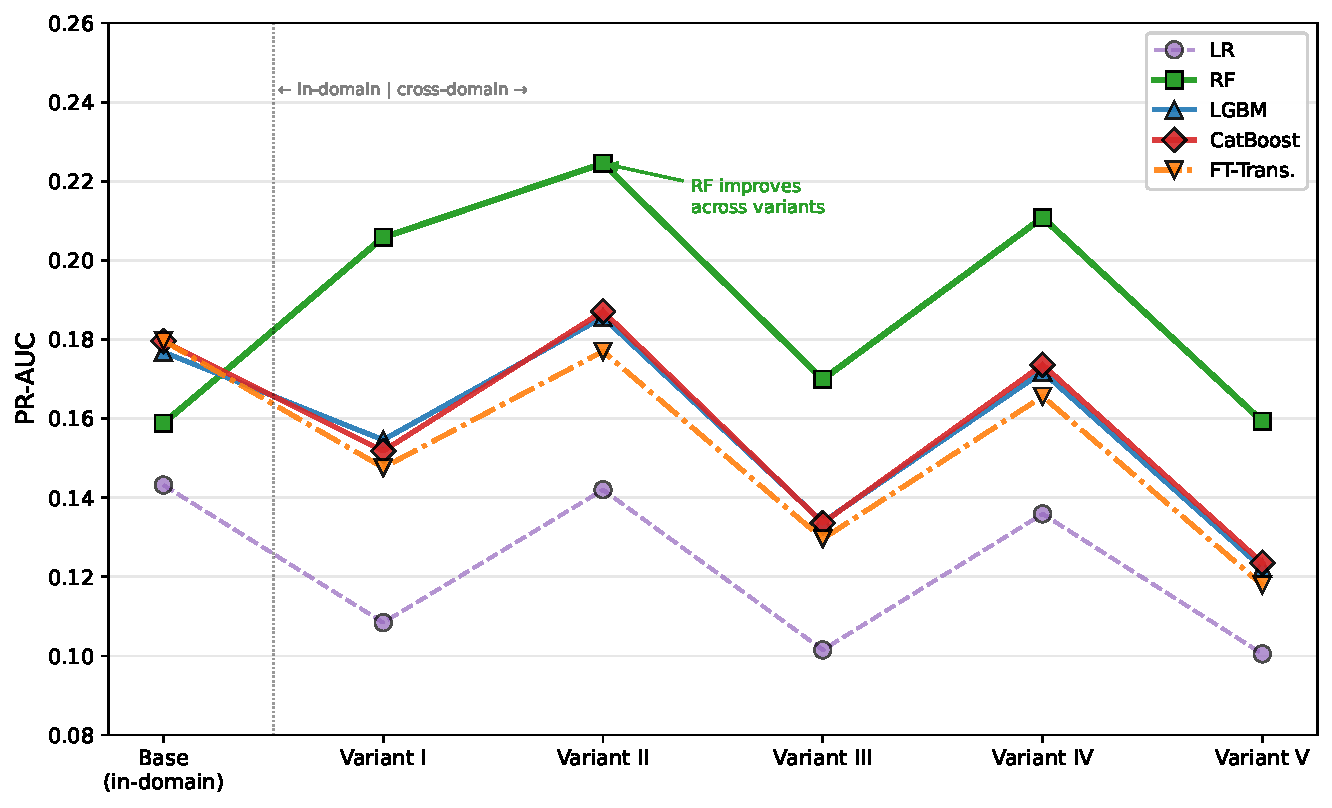
\includegraphics[width=0.92\textwidth]{figs/crossdomain_prauc.pdf}
\captionof{figure}{Cross-domain PR-AUC: models trained on BAF~Base and evaluated zero-shot on Variants~I--V.
  The dashed vertical line separates in-domain (Base) from cross-domain evaluation.
  Random Forest (green squares) is the only model that consistently improves relative to its Base score.}
\label{fig:crossdomain_prauc}
\end{minipage}

Three distinct response profiles emerge.
The first, shared by LGBM, CatBoost, and FT-Transformer, is one of
proportional degradation: Variant~II (label shift only) is recovered almost
perfectly, while Variants~III and~V (which combine covariate shift with
feature alignment changes) cause PR-AUC drops in the $24$--$34\%$ range.
Critically, FT-Transformer and CatBoost --- which tied at PR-AUC~$=\,0.180$
in-domain --- follow nearly identical degradation curves, ruling out any
cross-domain advantage for the attention-based architecture.

The second profile is Random Forest's, and it constitutes the most striking
finding of the cross-domain analysis.
Despite trailing LGBM and CatBoost in-domain by a substantial margin
($0.159$ vs.\ $0.177$--$0.180$ PR-AUC), Random Forest \emph{improves}
on four of the five variants.
On Variant~II it reaches PR-AUC~$=\,0.225$, exceeding the in-domain scores
of the gradient-boosted models.
In $F_2$ terms, RF improves from $0.294$ on Base to $0.319$ on Variant~II
and remains above its Base score on Variants~I, III, and~IV.
The third profile is OCSVM's: uniformly low across all variants (PR-AUC
below $0.023$), confirming the irrelevance of the one-class anomaly framing
on this benchmark.

ROC-AUC is notably more stable than PR-AUC across variants (range $0.87$--$0.91$
for supervised models), consistent with the known insensitivity of ROC-AUC
to class-prior shifts --- but for the same reason, a less discriminating metric
for model selection under extreme imbalance.

\subsection{Feature Attribution Analysis: SHAP}
\label{sec:shap}

Figure~\ref{fig:shap_global} shows the top-$15$ features by mean $|\text{SHAP}|$
for all four models on BAF~Base.

\noindent\begin{minipage}{\linewidth}\centering
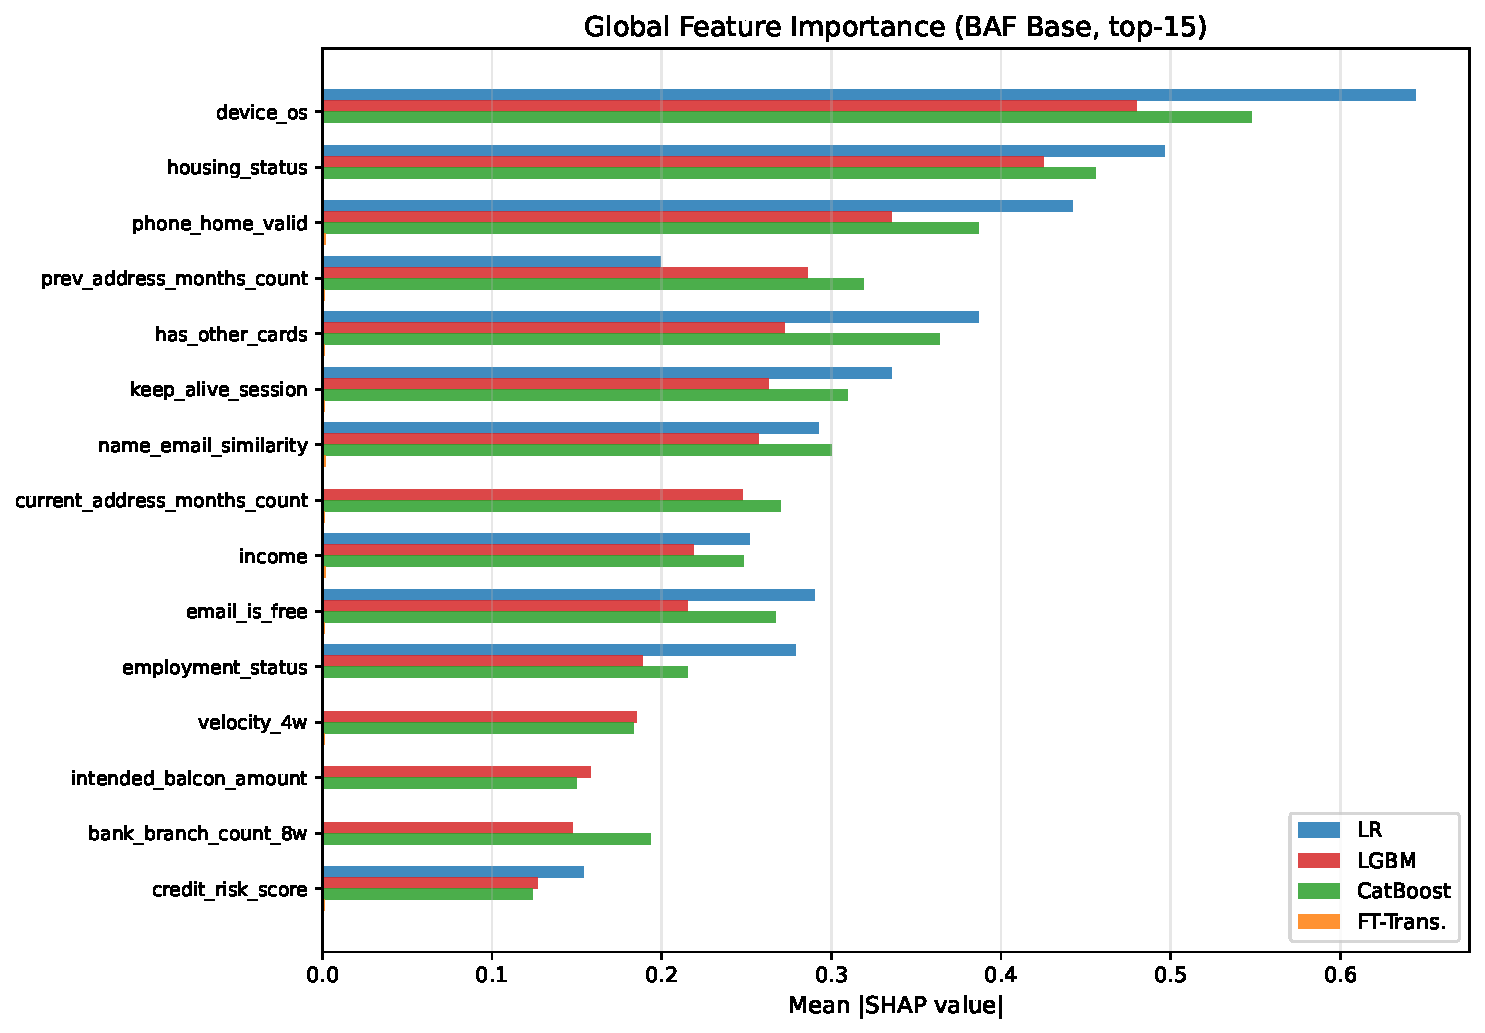
\includegraphics[width=0.90\textwidth]{figs/shap_global.pdf}
\captionof{figure}{Top-$15$ features by mean $|\text{SHAP}|$ on BAF~Base for LR,
  LGBM, CatBoost, and FT-Transformer. Tree-based models and LR concentrate on
  \texttt{device\_os}, \texttt{housing\_status}, and \texttt{phone\_home\_valid};
  FT-Transformer's top feature differs (\texttt{name\_email\_similarity}).}
\label{fig:shap_global}
\end{minipage}

LR, LGBM, and CatBoost agree on a compact set of three dominant features ---
\texttt{device\_os}, \texttt{housing\_status}, and \texttt{phone\_home\_valid}
--- which together occupy the top of every tree-based and linear ranking.
The FT-Transformer's leading feature is \texttt{name\_email\_similarity},
with \texttt{phone\_home\_valid} appearing third; only this single entry
is shared with the tree-based top.
Figure~\ref{fig:shap_beeswarm} details the LGBM attribution:
low values of \texttt{phone\_home\_valid} push strongly toward the fraud class,
while \texttt{device\_os} displays a discrete split with one category
concentrating most of the fraud signal --- a pattern consistent with a small
number of high-risk device fingerprints.

\noindent\begin{minipage}{\linewidth}\centering
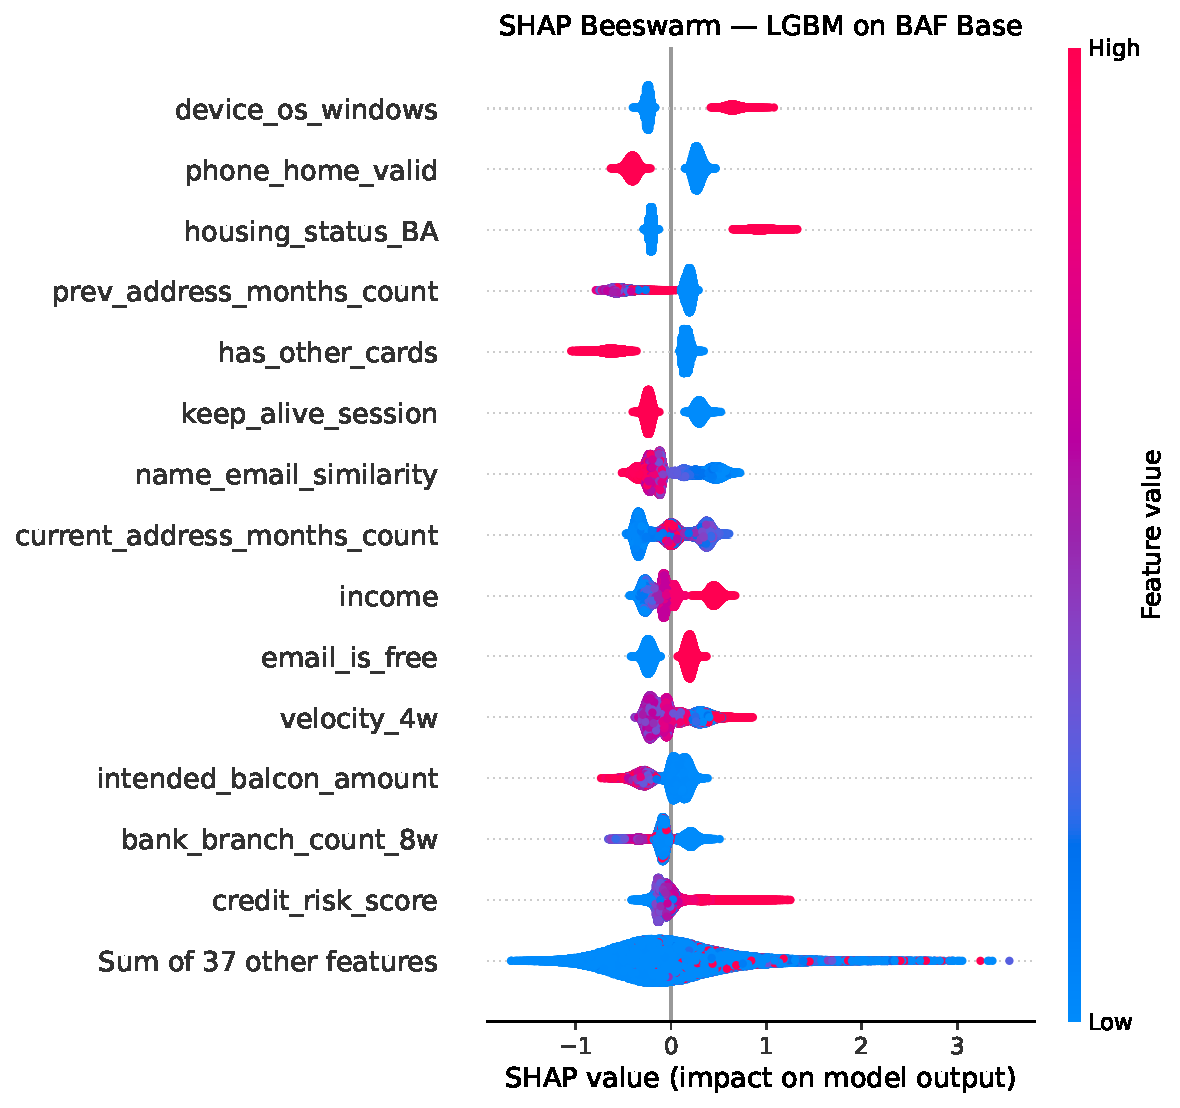
\includegraphics[width=0.90\textwidth]{figs/shap_beeswarm.pdf}
\captionof{figure}{SHAP beeswarm for LGBM on BAF~Base. Each dot is a test sample;
  red indicates high feature values, blue low. Features sorted by mean~$|\text{SHAP}|$.
  Low \texttt{phone\_home\_valid} and specific \texttt{device\_os} categories
  provide the strongest fraud signals.}
\label{fig:shap_beeswarm}
\end{minipage}

Table~\ref{tab:shap_consistency} reports pairwise Jaccard similarities of the
top-$10$ feature sets across all model pairs.

\noindent\begin{minipage}{\linewidth}\centering
\captionof{table}{Jaccard similarity of top-$10$ SHAP features across model pairs (BAF~Base).}
\label{tab:shap_consistency}
\begin{tabular}{l c c c c}
\toprule
          & LR   & LGBM & CatBoost & FT-Trans. \\
\midrule
LR        & ---  & 0.67 & 0.67 & 0.33 \\
LGBM      & 0.67 & ---  & 1.00 & 0.54 \\
CatBoost  & 0.67 & 1.00 & ---  & 0.54 \\
FT-Trans. & 0.33 & 0.54 & 0.54 & ---  \\
\bottomrule
\end{tabular}
\end{minipage}

LGBM and CatBoost agree perfectly on the top-$10$ feature set (Jaccard\,$=\,1.00$),
sharing seven of ten features with LR (Jaccard\,$=\,0.67$).
The FT-Transformer overlaps the tree-based ranking on five or six features
(Jaccard\,$=\,0.54$) and shares only three with LR (Jaccard\,$=\,0.33$).
This partial divergence does not imply worse predictive accuracy --- FT-Transformer
matches CatBoost at $0.180$ PR-AUC on BAF --- but it indicates that the transformer
learns a partially distinct feature hierarchy, weighting continuous features
more heavily than the discrete-valued categoricals that dominate tree-based rankings.

Table~\ref{tab:shap_stability} reports LGBM's top-$10$ feature stability
across all six BAF datasets.

\noindent\begin{minipage}{\linewidth}\centering
\captionof{table}{Jaccard similarity of LGBM's top-$10$ SHAP features across BAF variants.}
\label{tab:shap_stability}
\begin{tabular}{l c c c c c c}
\toprule
         & Base & Var.~I & Var.~II & Var.~III & Var.~IV & Var.~V \\
\midrule
Base      & ---  & 1.00 & 1.00 & 1.00 & 1.00 & 1.00 \\
Var.~I    & 1.00 & ---  & 1.00 & 1.00 & 1.00 & 1.00 \\
Var.~II   & 1.00 & 1.00 & ---  & 1.00 & 1.00 & 1.00 \\
Var.~III  & 1.00 & 1.00 & 1.00 & ---  & 1.00 & 1.00 \\
Var.~IV   & 1.00 & 1.00 & 1.00 & 1.00 & ---  & 1.00 \\
Var.~V    & 1.00 & 1.00 & 1.00 & 1.00 & 1.00 & --- \\
\bottomrule
\end{tabular}
\end{minipage}

The result is maximal: LGBM's top-$10$ feature ranking is identical on every BAF
dataset.
Combined with the cross-domain PR-AUC results, this constrains the source of
the observed degradation on Variants~III and~V: the features driving fraud
predictions are invariant under the distributional shifts of the BAF suite, so
any performance gap must come from changes in the relationship between those features
and the target label, not from a change in which features carry fraud signal.

Figure~\ref{fig:shap_waterfall} shows local SHAP contributions for representative
True Positive, False Positive, and False Negative cases.
The True Positive is supported by multiple features pushing concordantly toward fraud.
The False Positive shows the model constructing a near-fraud configuration from the
same features but with smaller individual contributions.
The False Negative --- the operationally most costly case --- has legitimate-pushing
features narrowly outweighing fraud indicators, producing a final score just below
threshold; from a practitioner perspective, recovering these FN cases would require
accepting a substantial precision penalty.

\noindent\begin{minipage}{\linewidth}\centering
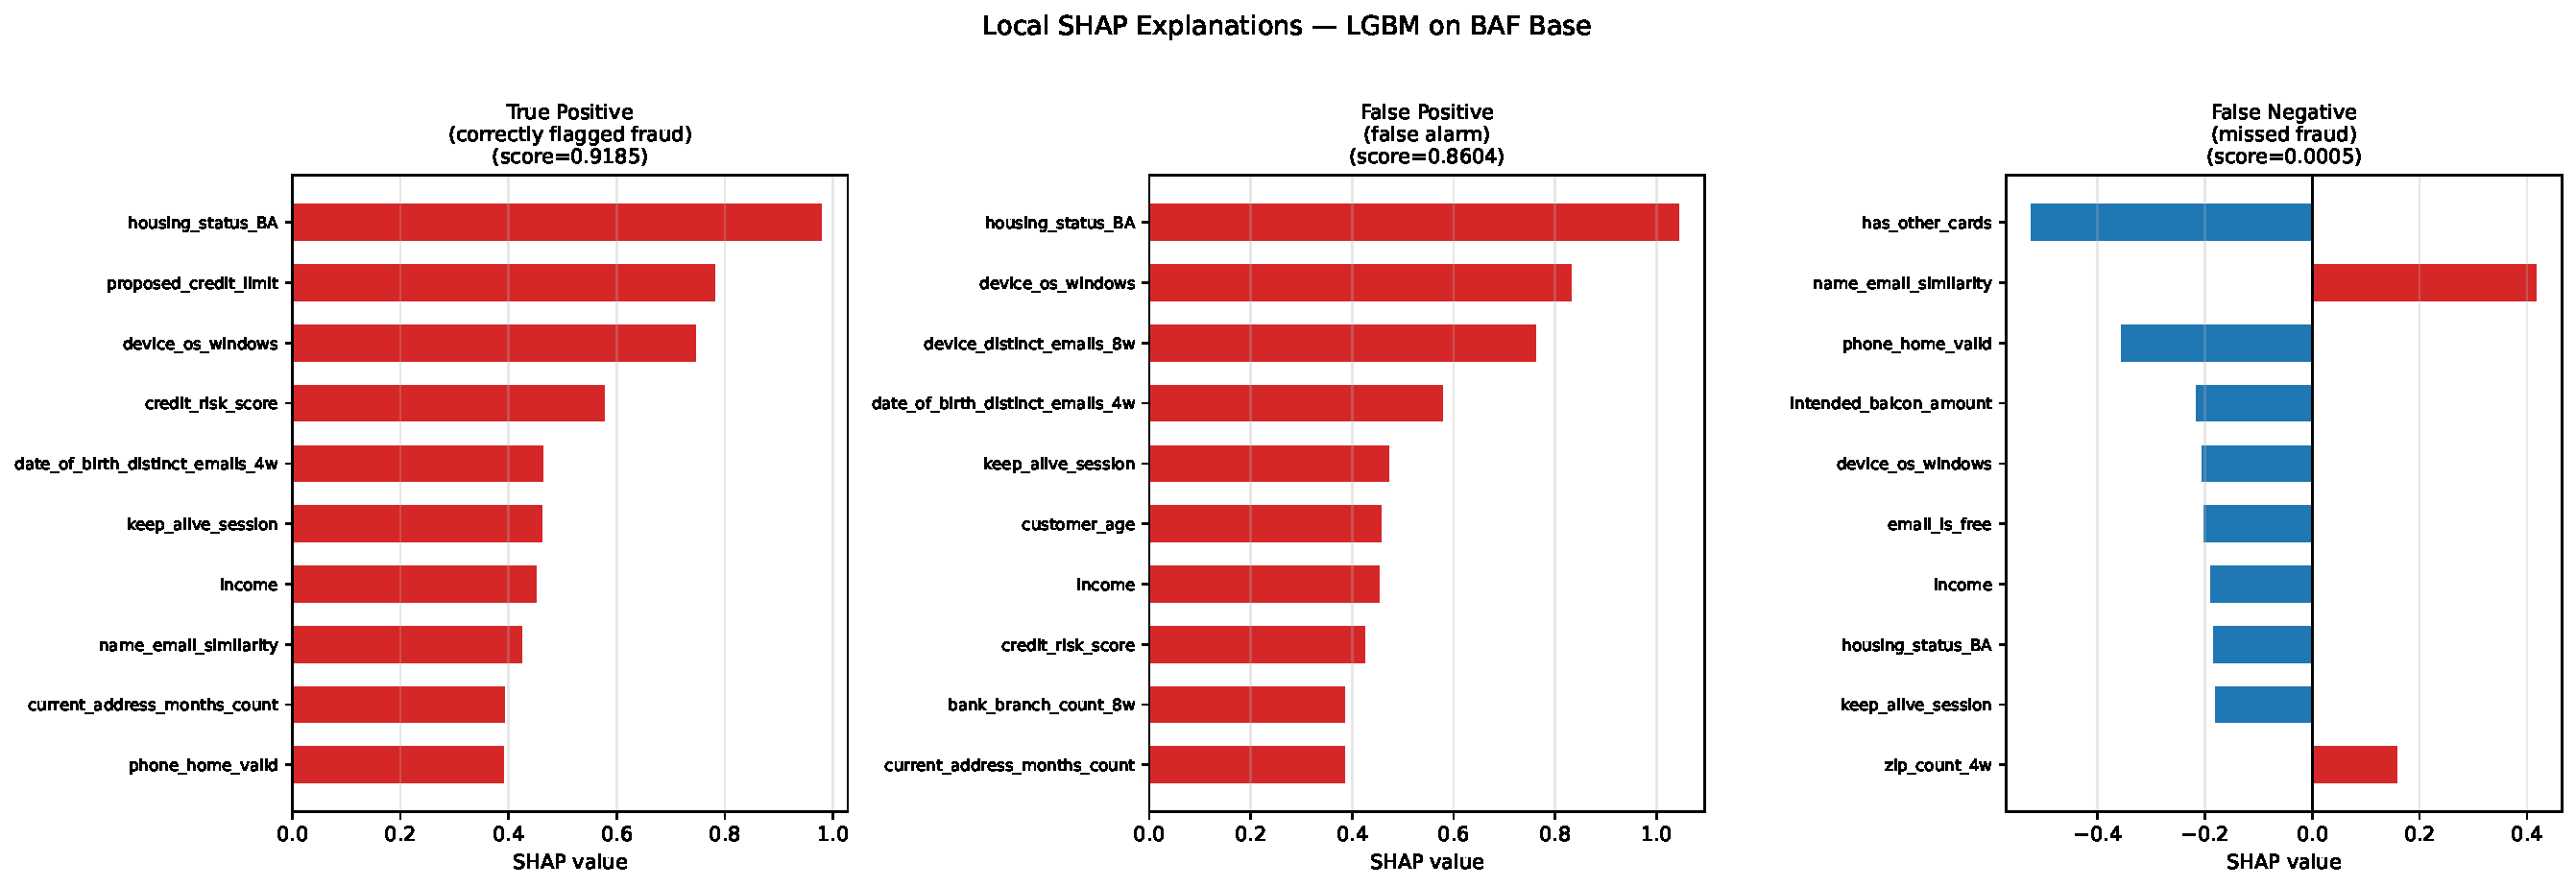
\includegraphics[width=0.95\textwidth]{figs/shap_waterfall.pdf}
\captionof{figure}{SHAP contribution plots for representative True Positive (left), False Positive (centre),
  and False Negative (right) cases (LGBM on BAF~Base).
  Red bars push toward fraud; blue bars push toward legitimate.}
\label{fig:shap_waterfall}
\end{minipage}

\subsection{FT-Transformer Attention Diagnostics: Foggy Vision}
\label{sec:attention}

Figure~\ref{fig:attention_aggregate} shows the mean attention weight per token
aggregated over all $200\,000$ BAF~Base test samples.

\noindent\begin{minipage}{\linewidth}\centering
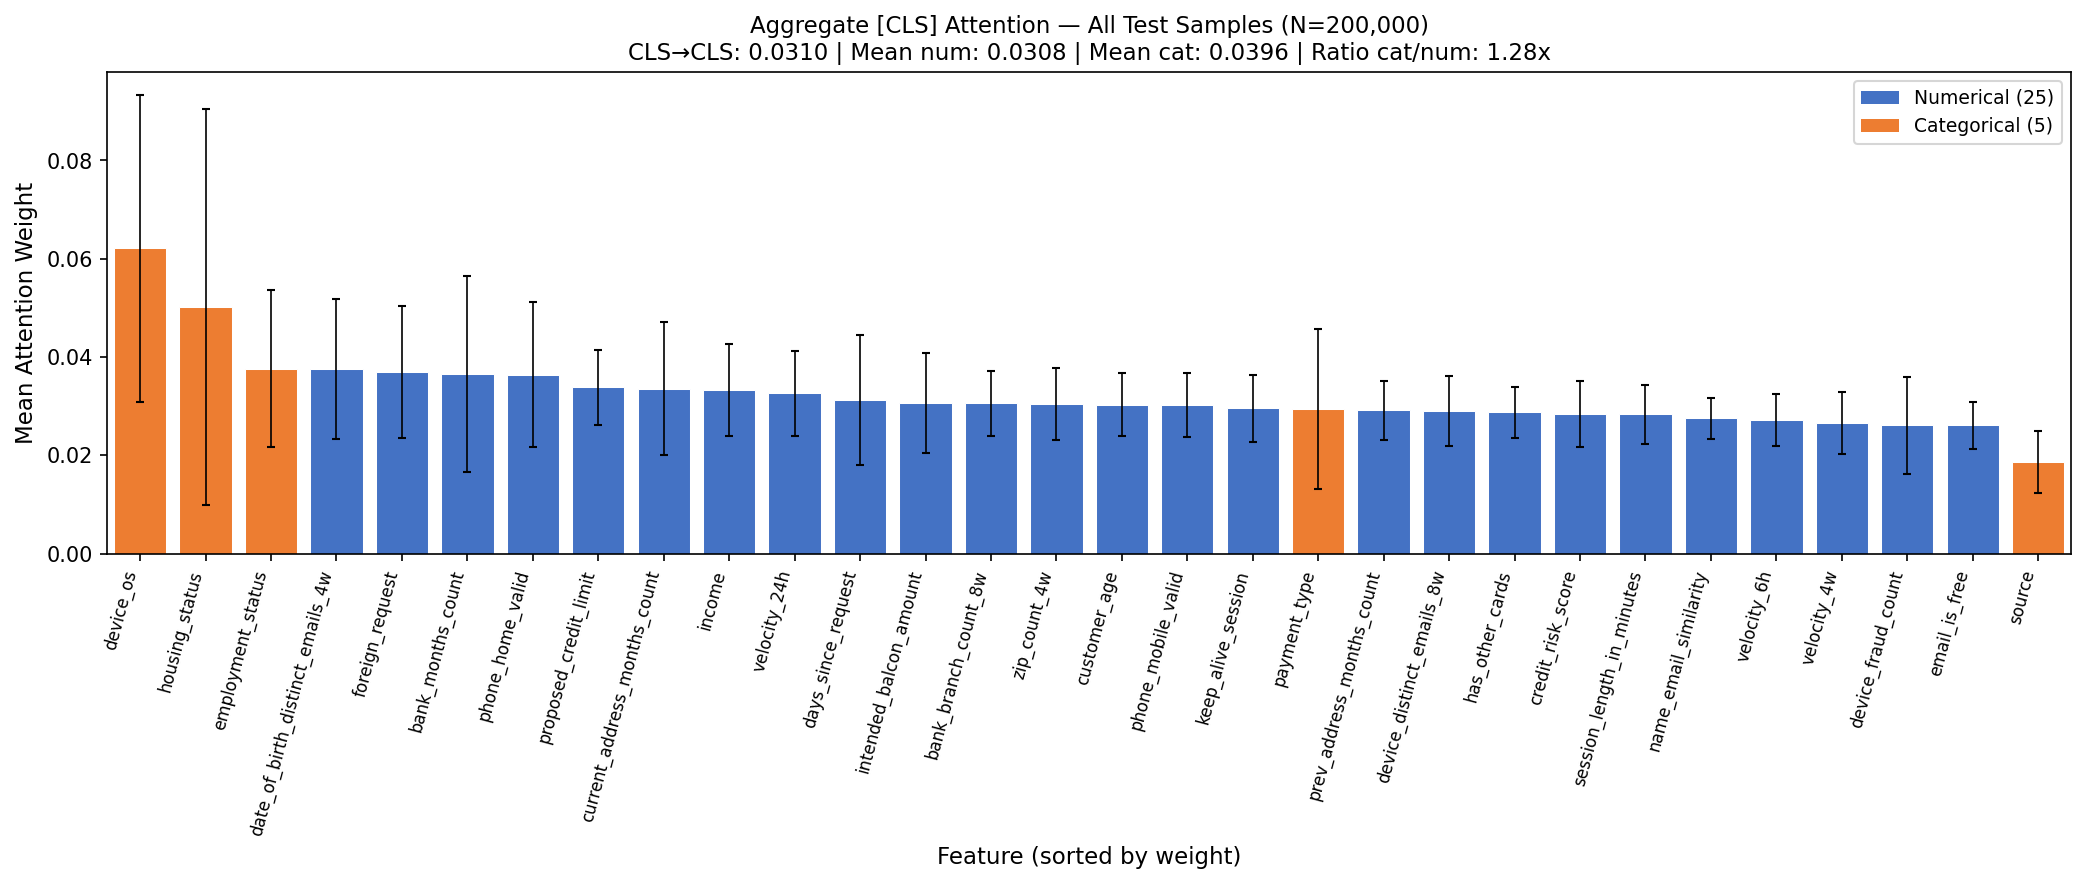
\includegraphics[width=0.95\textwidth]{figs/attention_aggregate.png}
\captionof{figure}{Mean attention weight per feature token over $200\,000$ BAF~Base test samples.
  Categorical features (orange) receive slightly higher attention than numerical ones (blue).
  The dashed reference line at $1/31 \approx 3.2\%$ marks the uniform baseline.
  Error bars show standard deviation across samples.}
\label{fig:attention_aggregate}
\end{minipage}

Four summary statistics characterise the aggregate distribution.
(i)~The normalised entropy is $H_{\text{norm}} = 0.976$, meaning the observed
entropy ($3.352$~nats) is $97.6\%$ of the theoretical maximum for $31$ tokens
($\ln 31 = 3.434$~nats): near-uniform attention across all tokens.
(ii)~The \texttt{[CLS]} self-attention is $3.1\%$, indistinguishable from the
uniform baseline of $1/31 \approx 3.2\%$, ruling out Self-Obsession.
(iii)~Mean categorical vs.\ numerical attention is $4.0\%$ vs.\ $3.1\%$
(ratio $1.28\times$), a small categorical elevation far below what constitutes
a Categorical Trap.
(iv)~The top three tokens by attention are \texttt{device\_os} ($6.2\%$),
\texttt{housing\_status} ($5.0\%$), and \texttt{employment\_status} ($3.8\%$),
precisely the three features that dominate the SHAP rankings of the tree-based
models (Section~\ref{sec:shap}).
The diagnostic verdict is \textbf{Foggy Vision}: none of Tunnel Vision,
Self-Obsession, or Categorical Trap is present.

Figure~\ref{fig:attention_heatmap_fp} shows the full $31\!\times\!31$ attention
matrix for a representative borderline False Positive case.

\noindent\begin{minipage}{\linewidth}\centering
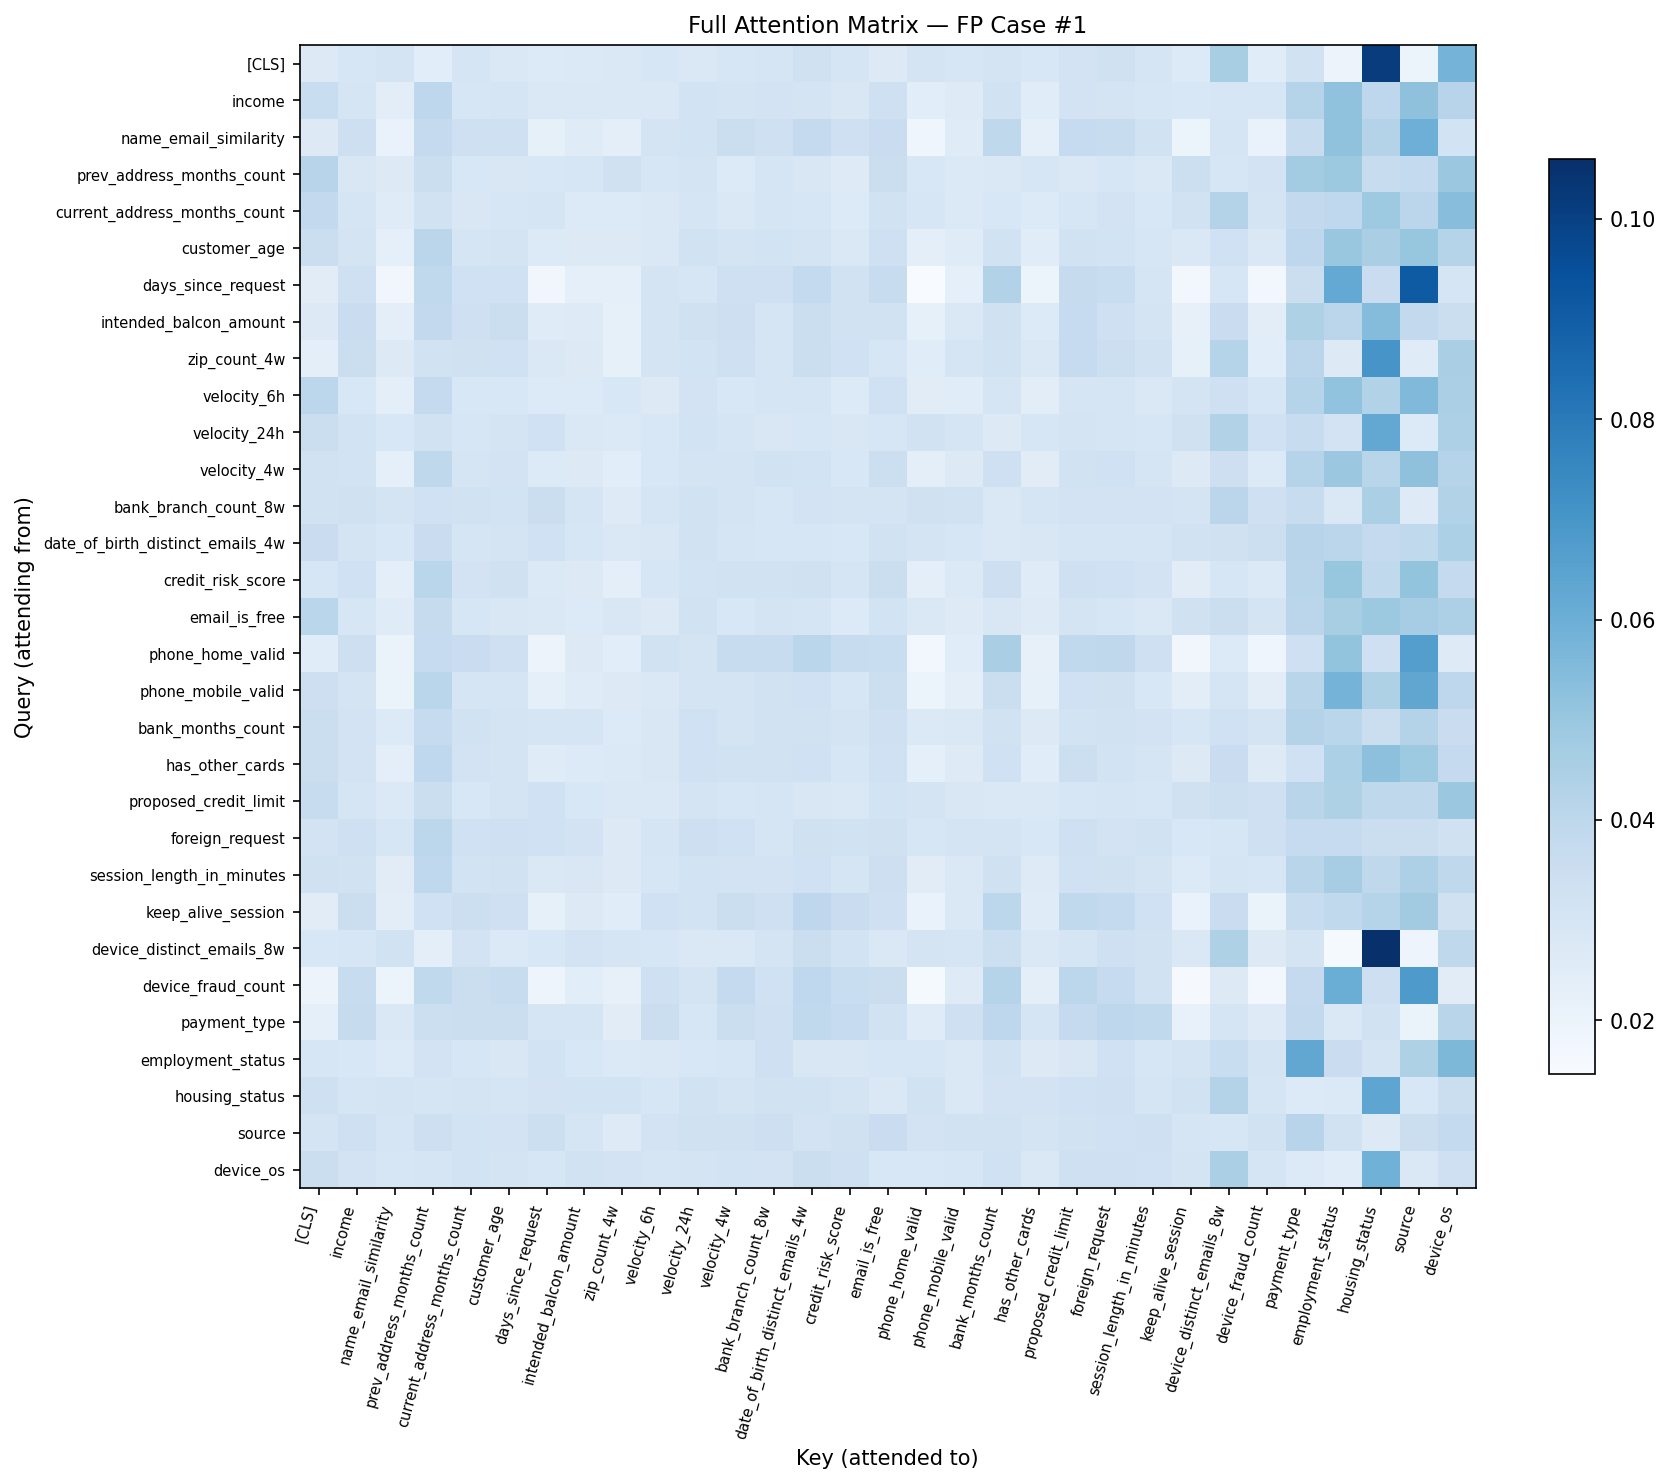
\includegraphics[width=0.80\textwidth]{figs/attention_heatmap_fp.png}
\captionof{figure}{Full $31\!\times\!31$ attention matrix for a representative False Positive case
  (score $\approx \tau = 0.058$).
  The near-uniform light-blue colouration across the entire matrix confirms the
  Foggy Vision pattern at the individual-case level.}
\label{fig:attention_heatmap_fp}
\end{minipage}

The individual heatmap confirms the aggregate finding: at the case level,
attention is dominated by near-uniform low values with only marginal concentration
on \texttt{device\_os} and \texttt{housing\_status}.
The classification in borderline cases is the product of a broad, distributed
aggregation of all $31$ feature representations, not a focused appeal to a
discriminative token.

%% ─── 5. Discussion ──────────────────────────────────────────────────────────

\section{Discussion}
\label{sec:discussion}

\subsection{Architectural Sensitivity to Synthetic Oversampling}
\label{sec:disc_smote}

The $41\%$ SMOTE-induced PR-AUC drop for FT-Transformer on BAF
(vs.\ $14\%$ for CatBoost) has a straightforward mechanistic interpretation.
SMOTE generates synthetic minority samples by linear interpolation between
existing fraud instances in the feature space~\citep{chawla2002smote}.
The FT-Transformer's attention mechanism processes each sample's feature
tokens and learns weights conditioned on the \emph{joint distribution} of
all $30$ features presented during training.
Synthetic interpolates alter this joint distribution: convex combinations
of rare fraud instances produce feature vectors that are geometrically feasible
but distributional anomalies --- combinations of feature values that do not
occur in the real data-generating process.
Attention layers trained on this distorted distribution generalise poorly
to test samples drawn from the genuine distribution, because the
per-feature attention weights are calibrated to the synthetic manifold rather
than the real one.

Tree-based models, by contrast, learn by axis-aligned splits on individual
feature values, not on continuous representations of the entire feature vector.
CatBoost's gradient boosting procedure is sensitive to the conditional distribution
of the target given each feature's splitting threshold, which is less distorted
by SMOTE interpolates than the global joint distribution seen by attention.
This explains both the asymmetry in the SMOTE effect and the fact that
Class Weights --- which modifies the loss function without altering the input
distribution --- is the safest intervention for FT-Transformer on both datasets.

On ULB, the reversal of the stability comparison (FT-T is marginally more stable
than CatBoost) is also explicable: ULB~2013's PCA-anonymised features
(V1--V28) have a well-separated, continuous structure where SMOTE interpolates
stay close to the genuine fraud manifold, so the joint-distribution distortion
is minor.
BAF's categorical-heavy feature space (five categorical features with binary
or low-cardinality values) is far more sensitive to interpolation: synthetic
samples created by averaging \texttt{device\_os} or \texttt{housing\_status}
values produce fractional encodings that are nonsensical in the original
feature space, amplifying the distributional mismatch for attention layers.

\subsection{Random Subsampling as Cross-Domain Regularization}
\label{sec:disc_rf}

The RF cross-domain superiority is, on its face, counter-intuitive: a model
that trails LGBM and CatBoost by $12$--$13\%$ in-domain PR-AUC improves on
four of five variants.
The explanation lies in RF's random feature subsampling ($\sqrt{p}$ features
considered at each split by default), which has a well-known regularizing
effect~\citep{breiman2001random}: each tree is forced to ignore a random subset
of features, preventing any single tree from learning an overly specialized
decision boundary that exploits feature co-occurrence patterns specific to the
training distribution.

LGBM and CatBoost grow trees on the global gradient signal, meaning their
boosted trees are allowed to use any feature combination at any split.
On BAF~Base, these models learn to exploit the joint configuration of
\texttt{device\_os}, \texttt{housing\_status}, and \texttt{phone\_home\_valid}
in a domain-specific way.
When the covariate distribution shifts (Variants~III, V) or the fraud
label assignment changes (Variants~I, II), those specific joint configurations
become less discriminative.
Random Forest's ``forced ignorance'' of features during each tree growth
is actually advantageous here: the resulting ensemble is less dependent on
any particular feature combination and therefore more resilient when those
combinations shift.
This finding has a practical implication that runs counter to common practice:
\emph{a lower in-domain score is not a reliable proxy for cross-domain robustness};
when distribution shift is anticipated at deployment, RF should be the primary
model candidate, not the highest in-domain scorer.

The cross-domain threshold transfer is also noteworthy: the threshold $\tau$
calibrated on the Base validation fold applies to all variants without recalibration.
On Variants~I and~II (where RF improves), this means that the
threshold calibrated at Base prevalence remains appropriate under variant conditions.
This is consistent with the SHAP stability finding: if the feature distributions
that drive predictions are unchanged (Jaccard\,$=\,1.00$ for LGBM), the optimal
threshold for a given feature configuration is stable across variants.

\subsection{Feature Attribution Stability as a Diagnostic Instrument}
\label{sec:disc_shap}

The Jaccard\,$=\,1.00$ result for LGBM across all six BAF datasets is the most
informative of the stability findings.
It does not mean that fraud is equally detectable on all variants --- it means
that \emph{the same features carry the fraud signal regardless of which variant
is evaluated}.
The performance degradation on Variants~III and~V ($0.177 \to 0.134$ PR-AUC for LGBM)
therefore does not arise from the model suddenly relying on different features;
instead, it arises from a change in the \emph{conditional relationship} between
those stable features and the fraud label --- which is precisely what covariate
and label shift alter by design in the BAF suite.

This diagnostic capability has an immediate practical consequence: explanations
generated on the training distribution remain valid on shifted variants.
A fraud analyst relying on LGBM explanations to understand model decisions
does not need to regenerate the SHAP infrastructure when the model encounters
Variant~I or Variant~II data; the same features, in the same order, drive the same
predictions.
The FT-Transformer's lower Jaccard similarity with tree-based models ($0.54$)
is more nuanced: it does not indicate that FT-Transformer explanations are wrong,
but rather that the transformer emphasises continuous features
(\texttt{name\_email\_similarity}, \texttt{income}) more strongly than the
categorical features that dominate tree-based rankings.
This is consistent with FT-Transformer's tokenisation design, which applies a
learned linear projection to each numerical feature, providing richer gradient
signal from continuous inputs than from one-hot categorical embeddings.

\subsection{Convergent Validity and the Dataset Ceiling Interpretation}
\label{sec:disc_ceiling}

The convergent validity finding --- that attention top tokens and SHAP top features
agree on the same three primary signals (\texttt{device\_os}, \texttt{housing\_status},
\texttt{phone\_home\_valid}) --- is a stronger guarantee than either method alone
could provide.
Attention weights can be confounded by architectural biases (e.g.\ higher attention
to tokens with larger embedding norms); SHAP values can be confounded by feature
correlations (e.g.\ TreeExplainer vs.\ GradientExplainer making different independence
assumptions).
When two structurally different methods produce the same feature ranking on the
same data, the conclusion that these features carry genuine, robust fraud signal
is substantially more credible than if it rested on either method in isolation.

The Foggy Vision pattern ($H_{\text{norm}} = 0.976$) provides the final interpretive
piece.
FT-Transformer achieves $0.18$ PR-AUC on BAF --- identical to CatBoost --- not
because its attention mechanism is broken, degenerate, or miscalibrated.
The model integrates information from all $31$ tokens nearly uniformly precisely
because the BAF feature space does not reward selective attention: there is no
small subset of tokens that, if attended to, would yield substantially better
predictions.
The performance ceiling at $0.18$ PR-AUC is therefore a property of the feature
space and the label generating process, not of any model's inadequacy.
This interpretation is consistent with: (i) the perfect SHAP cross-variant stability
(no new features emerge as discriminative on shifted variants), (ii) the
statistical indistinguishability of CatBoost and FT-Transformer bootstrap CIs
reported in~\citet{caixeiro2025threshold}, and (iii) the negligible categorical
attention preference ($1.28\times$) which, while mechanistically expected from
FT-Transformer's tokenisation, does not translate into any measurable performance
advantage.

The practical implication is sobering but important: on BAF data with these
$30$ features, adding a more powerful model, applying a novel resampling strategy,
or extending the attention architecture is unlikely to push PR-AUC substantially
above $0.18$.
Progress on this benchmark will require either additional informative features
or a different modelling of the fraud-generating process.

%% ─── 6. Conclusion ──────────────────────────────────────────────────────────

\section{Conclusion}
\label{sec:conclusion}

This paper provided a mechanistic account of why gradient-boosted decision trees
generalise better than tabular transformers under distribution shift in financial
fraud detection.
Four complementary analyses on the BAF suite showed that: SMOTE degrades
FT-Transformer PR-AUC by $41\%$ on BAF because synthetic interpolates distort
the joint feature distribution that attention relies on (vs.\ $14\%$ for CatBoost,
whose split-based learning is less sensitive to global distribution shape);
Random Forest improves on four of five BAF cross-domain variants despite a lower
in-domain score, because random feature subsampling prevents over-specialisation
to base-domain feature co-occurrence patterns; LGBM's SHAP top-$10$ feature ranking
is perfectly stable (Jaccard\,$=\,1.00$) across all six BAF datasets, confirming
that observed performance degradation under shift reflects changes in the
feature--label relationship rather than the features themselves;
and FT-Transformer's near-uniform attention (entropy $0.976$, Foggy Vision)
rules out all pathological attention patterns and confirms that the $0.18$
PR-AUC ceiling on BAF is a signal-space ceiling, not an architectural failure.
Convergent validity between SHAP and attention --- both pointing to the same three
primary fraud signals --- strengthens confidence in the explanations produced by
either method independently.

For practitioners, the principal recommendations are: prefer CatBoost or LGBM
for in-domain deployment on BAF-scale data; choose RF when cross-domain robustness
is the primary concern; avoid SMOTE for FT-Transformer and use Class Weights
instead; rely on LGBM SHAP explanations across distributional variants without
recomputation.

Two limitations bound these conclusions.
First, both datasets are either PCA-anonymised (ULB) or synthetically generated (BAF),
so findings may not transfer to production fraud streams with richer feature semantics,
adversarial label noise, or temporal feedback loops.
Second, the attention diagnostic is computed on a single FT-Transformer
configuration; the Foggy Vision pattern may not generalise to architectures with
more attention heads, deeper stacks, or different tokenisation strategies.
A natural extension is to apply the same diagnostic framework to additional
tabular transformer architectures (SAINT, TabTransformer) and to real-world
fraud datasets where the feature-space ceiling can be tested against independent
external evidence.

\section*{CRediT authorship contribution statement}

\textbf{Olavo Caixeiro}: Conceptualization, Methodology, Software, Formal analysis,
  Writing -- original draft. \\
\textbf{Maryam Abbasi}: Conceptualization, Supervision, Writing -- review \& editing. \\
\textbf{Pedro Martins}: Supervision, Writing -- review \& editing.

\section*{Declaration of Competing Interests}

The authors declare that they have no known competing financial interests or personal
relationships that could have appeared to influence the work reported in this paper.

\section*{Data Availability}

The ULB~2013 dataset is publicly available at Kaggle (Credit Card Fraud Detection).
The BAF suite is publicly available from the authors of~\citet{jesus2022turning}
at \texttt{https://github.com/feedzai/bank-account-fraud}.
Experimental code and results are available upon reasonable request from the
corresponding author.

%% ─── Bibliography ───────────────────────────────────────────────────────────

\bibliographystyle{cas-model2-names}
\bibliography{cas-refs}

\end{document}
